\documentclass[../statistical_learning_notes.tex]{subfiles}
\begin{document}
    %%%%%%%%%%%%%%%%%%%%%%%%%%%%%%%%%%%%%%%%%%%%%%%%%%%%%%%%%%%%%%%%%%%%%%%%%%%%%%%
    \chapter{Support Vector Machines}
    Maximal margin classifier is the first idea for the development towards SVMs. Maximal margin classifier utilizes hyperplanes and requires that the data is linearly separable. The extension of this is Support Vector Classifier that can be applied to an even broader class of problems where classes may not be perfectly separable. SVMs are a further extension of SVCs to account for non linear separation boundaries.

    \paragraph{Hyperplane} in a $p$-dimensional space is a surface that is an affine subspace (means it need not pass through origin) in the $p-1$ dimensional space. For a 2D space it will be a 1D line, for a 3D space it will be a 2D plane, and so on. The equation is of the form
    \begin{align*}
        \beta_{0} + \beta_{1}X_{1} + \beta_{2}X_{2} + \cdots + \beta_{p}X_{p} = 0
    \end{align*}
    Any point in the vector space can fall into one of the three regions
    \begin{align*}
        \beta_{0} + \beta_{1}X_{1} + \beta_{2}X_{2} + \cdots + \beta_{p}X_{p} \begin{cases}
            > 0\\
            = 0\\
            > 0
        \end{cases}
    \end{align*}
    and thus a hyperplane can be a useful demarcation between two regions or classes.\newline

    From now on, let $\beta^{T} = (\beta_{1}, \ldots, \beta_{p})$, $x^{T} = (x_{1}, \ldots, x_{p})$, $\beta_{0}$ be a scalar, and $N$ denote the total number of training data points. Although not represented by a bold font, $\beta$ and $x$ are both vectors. Since $\beta^{T}x$ is a scalar, $\beta^{T}x = x^{T}\beta$.
    

    %%%%%%%%%%%%%%%%%%%%%%%%%%%%%%%%%%%%%%%%%%%%%%%%%%%%%%%%
    \section{Maximal Margin Classifier}
    Maimum Margin Classifier uses hyper planes to find a separable boundary between linearly separable data points.\newline

    Suppose we have a set of data points with $p$ predictors and they belong to two classes given by $y_{i} = \{-1 , 1\}$. Suppose the points are perfectly separable through a hyperplane. Then the following hold
    \begin{alignat*}{2}
        &\beta_{0} + \beta^{T}x_{i} &&> 0 \quad \text{when} \quad y_{i} = -1\\
        \text{and} \quad &\beta_{0} + \beta^{T}x_{i} &&< 0 \quad \text{when} \quad y_{i} = 1\\
        \implies y_{i}(&\beta_{0} + \beta^{T}x_{i}) &&> 0
    \end{alignat*}

    Thus classification can be made into the positive or negative class simply based on the sign of the quantity $\beta^{T}x$. The further a point is, the more confident we will be in the classification.\newline

    Note that there can be infinite such hyperplanes that perfectly separate the data, and each can be obtained by slightly perturbing the given plane. Define margin as the minimum perpendicular distance from all training observations to this plane. The maximum margin classifier will be the one for which this margin is maximum.\newline

    \begin{figure}[h]
    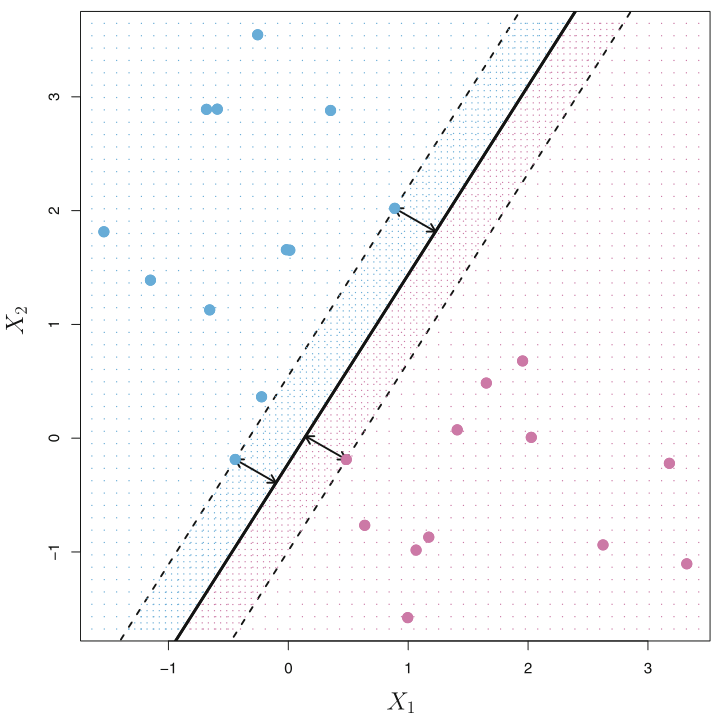
\includegraphics[scale=0.6]{mmc}
    \centering
    \caption{The Maximal Margin Classifier with the Support Vectors. Dotted lines represent the margin.}
    \label{fig:mmc} %\ref{fig:mmc}
    \end{figure}

    Note that the location of the maximal margin is determined only by the points closest to the boundary. If a point farther away would slightly move, the boundary would still be the same. Whereas if the point closer to the boundary would shift, the boundary itself would change as can be seen in figure \ref{fig:mmc}. These set of observations are know as \textbf{support vectors}. And by symmetry, the perpendicular distances of these closest points from the plane are same.

    
    %%%%%%%%%%%%%%%%%%%%%%%%%%%%%%%%%%%
    \subsection{Algorithm}
    Finding the boundary is same as solving for the following optimization problem ($M$ is the margin)
    \begin{align*}
        &\maximize_{\beta_{0}, \beta} M\\
        &\text{subject to} \quad \sum_{i=1}^{p} \beta_{i}^{2} = 1,\\
        &\text{and} \quad y_{i}(\beta_{0} + \beta^{T}x_{i}) \geq M \quad \forall \quad i = 1, 2, \ldots, N
    \end{align*}
    The constraint $\sum_{i=1}^{p} \beta_{i}^{2} = 1$ gives rise to the unique property that $\beta_{0} + \beta^{T}x$ is the perpendicular distance of the point $x$ from the hyperplane, making the last constraint equation valid. The proof of the perpendicular distance equation is given in section \ref{sec:appendix_mmc_perpendicular_dist}.\newline

    By using the perpendicular distance using the equation from section \ref{sec:appendix_mmc_perpendicular_dist}, we can replace the constraint on the norm and rewrite as
    \begin{gather*}
        \maximize_{\beta_{0}, \beta} M\\
        \text{subject to} \quad y_{i}(\beta_{0} + \beta^{T}x_{i}) \geq M \lVert \beta \rVert \quad \forall \quad i = 1, 2, \ldots, N
    \end{gather*}

    Note that the last equation remains same when we multiply by a positive constant. Hence, we can choose $\lVert \beta \rVert = 1/M$ for simplicity and the maximization problem becomes a minimization one (a factor of $1/2$ is introduced to simplify the derivative of the square term)
    \begin{gather*}
        \minimize_{\beta_{0}, \beta}  \frac{1}{2}\lVert \beta \rVert^{2}\\
        \text{subject to} 1 - \quad y_{i}(\beta_{0} + \beta^{T}x_{i}) \leq 0 \quad \forall \quad i = 1, 2, \ldots, N
    \end{gather*}

    For the following derivations involving linear optimization, refer to appendix (section \ref{sec:appendix_lagrangian}).\newline
    Invoking the Lagrangian multipliers, the new optimization problem is
    \begin{align*}
        \minimize_{\beta_{0},\beta}  \frac{1}{2}\lVert \beta \rVert^{2} - \sum_{j=1}^{N} \lambda_{j} (y_{j}(\beta_{0} + \beta^{T}x_{j}) - 1)
    \end{align*}

    where $\lambda = (\lambda_{1}, \ldots \lambda_{N})^{T}$. Using the Wolfe Dual, the following is the dual problem

    \begin{gather*}
        \maximize_{\beta, \beta_{0}, \lambda} L(\beta, \beta_{0}, \lambda) = \frac{1}{2}\lVert \beta \rVert^{2} - \sum_{j=1}^{N} \lambda_{j} (y_{j}(\beta_{0} + \beta^{T}x_{j}) - 1)\\
        \text{subject to} \quad \lambda > 0, \quad \frac{\partial L}{\partial \beta} = 0 \quad \text{and} \quad \frac{\partial L}{\partial \beta_{0}} = 0
    \end{gather*}

    The partial derivatives give
    \begin{align*}
        \beta = \sum_{j=1}^{N} \lambda_{j} y_{j}x_{j} \quad \text{and} \quad 0 = \sum_{j=1}^{N}\lambda_{j} y_{j}
    \end{align*}

    Substituiting in the dual,
    \begin{align*}
        L(\lambda) &= \frac{1}{2}\beta^{T} \beta - \sum_{j=1}^{N} \lambda_{j} (y_{j}(\beta_{0} + \beta^{T}x_{j}) - 1)\\
        &= \frac{1}{2}\beta^{T} \beta - \beta_{0}(\sum_{j=1}^{N} \lambda_{j} y_{j}) - \beta^{T}(\sum_{j=1}^{N} \lambda_{j} y_{j} x_{j}) + \sum_{j=1}^{N}\lambda_{j}\\
        &= \frac{1}{2}\beta^{T} \beta - \beta_{0}(0) - \beta^{T} \beta + \sum_{j=1}^{N}\lambda_{j}\\
        &= \sum_{j=1}^{N}\lambda_{j} - \frac{1}{2}\beta^{T} \beta
        = \sum_{j=1}^{N}\lambda_{j} - \frac{1}{2}(\sum_{i=1}^{N} \lambda_{i} y_{i}x_{i}^{T})(\sum_{j=1}^{N} \lambda_{j} y_{j}x_{j})\\
        &= \sum_{j=1}^{N}\lambda_{j} - \frac{1}{2} \sum_{i=1}^{N} \sum_{j=1}^{N} \lambda_{i} \lambda_{j} y_{i}y_{j}x_{i}^{T}x_{j}
    \end{align*}

    along with the constraints,
    \begin{gather*}
        \maximize_{\lambda} \sum_{j=1}^{N}\lambda_{j} - \frac{1}{2} \sum_{i=1}^{N} \sum_{j=1}^{N} \lambda_{i} \lambda_{j} y_{i}y_{j}x_{i}^{T}x_{j}\\
        \text{subject to} \quad \lambda > 0 \quad \text{and} \quad 0 = \sum_{j=1}^{N}\lambda_{j} y_{j}
    \end{gather*}

    which is a quadratic optimization problem with linear constraints, and is solvable through linear optimization softwares. Maximizing the the dual will give us the lower bound of the optimal solution.\newline

    KKT conditions also need to be satisfied for the optimal solution, which gives
    \begin{gather*}
        \lambda_{j}^{*} (y_{j}(\beta_{0}^{*} + \beta^{*T}x_{j}) - 1 = 0 \quad \forall \: j = 1, 2, \ldots N\\
        \implies y_{j}(\beta_{0}^{*} + \beta^{*T}x_{j}) - 1 = 0 \quad \text{for points on margin}\\
        \lambda_{j}^{*} = 0 \quad \text{for points away from the margin}
    \end{gather*}
    which is expected based on the definition of the problem as only the points on margin decide the separating hyperplane. The predictions for new data points are simply made on the basis of the sign of $\beta_{0}^{*} + \beta^{*T}x$


    %%%%%%%%%%%%%%%%%%%%%%%%%%%%%%%%%%%%%%%%%%%%%%%%%%%%%%%%
    \section{Support Vector Classifier}
    The previous section was the best case scenario when all observations are perfectly separable. But in real data, this is seldom the case and we encounter the scenario that some observations will be misclassified. To take this into account, we maintain the same optimization as the previous section, but introduce new slack variables to account for the misclassified points
    \begin{align*}
        &\maximize_{\beta_{0},\ldots,\beta_{p}, M} M\\
        &\text{subject to} \quad \sum_{i=1}^{p} \beta_{i}^{2} = 1,\\
        &\text{and} \quad y_{i}(\beta_{0} + \beta_{1}x_{i1} + \cdots + \beta_{p}x_{ip}) \geq M(1-\epsilon_{i}) \quad \forall \quad i = 1, 2, \ldots, n\\
        &\epsilon_{i} > 0, \sum_{i=1}^{n}\epsilon_{i} \leq C
    \end{align*}

    which simply means that if
    \begin{enumerate}
        \item $\epsilon_{i} = 0$, we have correctly classified the observation
        \item $\epsilon_{i} < 1$, the observation is correctly classified, but lies between the hyperplane and the margin, thus violating the margin
        \item $\epsilon_{i} > 1$, the observation is misclassified
    \end{enumerate}
    The term $C$ is tells how much of the margin we have violated. Observations on the correct side of the margin will have no contribution to this value. Only the ones violating the margin or the hyperplane will contribute.\newline

    Another thing to notice is the use of $M(1-\epsilon)$ in the inequality instead of simply$M - \epsilon$. The first term denots the relative difference in margin while the second term gives the actual difference. Both the formulations lead to different solutions as the former is convex optimization and the latter is non convec. Further, using the former, we can formulate the problem in a manner similar to the maximum margin classifier

    \begin{gather*}
        \minimize_{\beta_{0}, \beta}  \frac{1}{2}\lVert \beta \rVert^{2} + C\sum_{j=1}^{N}\epsilon_{j}\\
        \text{subject to} \quad (1-\epsilon_{j}) - y_{i}(\beta_{0} + \beta^{T}x_{i}) \leq 0, \: -\epsilon \leq 0 \quad \forall \quad i = 1, 2, \ldots, N\\
    \end{gather*}
    Replacing the constraint on the sum of the slack variables with a simple $C * sum$ is similar to one done in ridge or lasso shrinkages (section \ref{sec:alternative_ridge_lasso}). $C$ is a constant and will limit how much error we are wiling to tolerate. $C = \inf$ gives us the original separable case since that forces all the $\epsilon$ to be $0$. As we decrease $C$, the epsilons are allowed to take larger values we are allowing more points to be misclassified leading to narrower margins (figure \ref{fig:svm_1}).\newline

    \begin{figure}[h]
    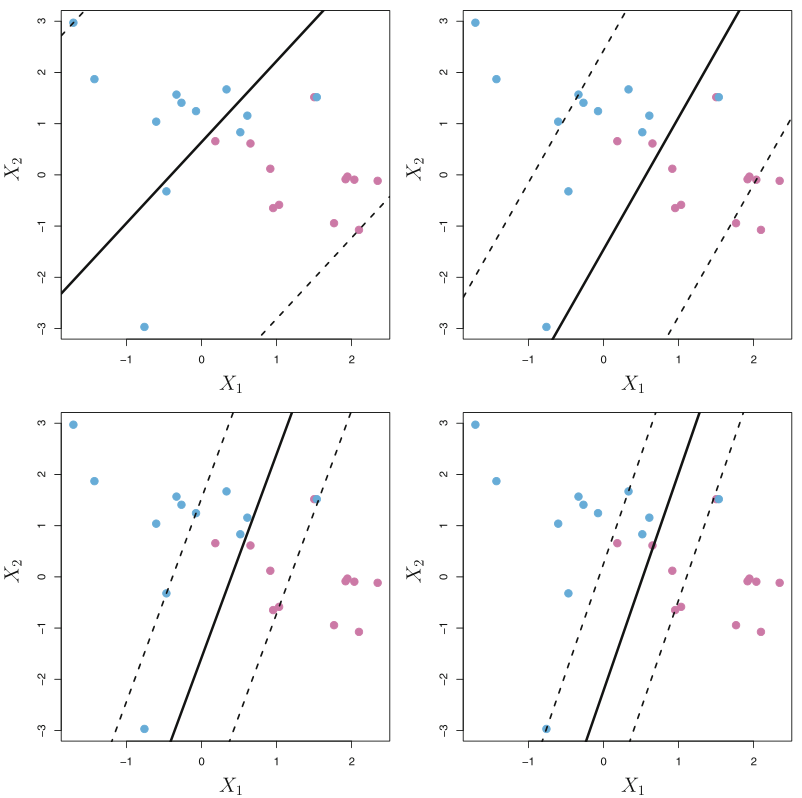
\includegraphics[scale=0.6]{svm_1}
    \centering
    \caption{Support Vector Classifier with decreasing $C$ from top left to bottom right causing narrowing margins.}
    \label{fig:svm_1} %\ref{fig:svm_1}
    \end{figure}

    The Lagrangian becomes
    \begin{gather*}
        L = \frac{1}{2}\lVert \beta \rVert^{2} + C\sum_{j=1}^{N}\epsilon_{j} + \sum_{j=1}^{N} \lambda_{j}((1-\epsilon_{j}) - y_{i}(\beta_{0} + \beta^{T}x_{i})) + \sum_{j=1}^{N} \mu_{j}(-\epsilon_{j})
    \end{gather*}
    where $\lambda = (\lambda_{1}, \ldots, \lambda_{N})^{T}$, $\mu = (\mu_{1}, \ldots, \mu_{N})^{T}$ and $\epsilon = (\epsilon_{1}, \ldots, \epsilon_{N})^{T}$ and the Wolfe Dual is (all functions in $L$ are differentiable)
    \begin{gather*}
        \max_{\beta_{0}, \beta, \epsilon} L\\
        \text{subject to} \quad \lambda > 0, \; \mu>0, \; \frac{\partial L}{\partial \beta} = 0, \; \frac{\partial L}{\partial \beta_{0}} = 0, \; \frac{\partial L}{\partial \epsilon_{j}} = 0
    \end{gather*}

    The derivatives equations give the following results
    \begin{gather*}
        \frac{\partial L}{\partial \beta} = 0 \; \implies \beta - \sum_{j=1}^{N}\lambda_{j}y_{j}x_{j} = 0\\
        \frac{\partial L}{\partial \beta_{0}} = 0 \; \implies \sum_{j=1}^{N} \lambda_{j}y_{j} = 0\\
        \frac{\partial L}{\partial \epsilon_{j}} = 0 \; \implies C - \lambda_{j} - \mu_{j} = 0
    \end{gather*}

    Substituiting in the dual leaves us with only $\lambda$ as the variable
    \begin{align*}
        L &= \frac{1}{2}\beta^{T}\beta + C\sum_{j=1}^{N}\epsilon_{j} + \sum_{j=1}^{N}\lambda_{j}(1 - \epsilon_{j}) - \beta^{T}(\sum_{j=1}^{N} \lambda_{j}y_{j}x_{j}) - \beta_{0}\sum_{j=1}^{N}\lambda_{j}y_{j} - \sum_{j=1}^{N}(C - \lambda_{j})\epsilon_{j}\\
        &= \frac{1}{2}\beta^{T}\beta + \sum_{j=1}^{N}\lambda_{j} -\beta^{T}\beta = -\frac{1}{2}\beta^{T}\beta + \sum_{j=1}^{N}\lambda_{j}\\
        &= \sum_{j=1}^{N}\lambda_{j} - \frac{1}{2} \sum_{i=1}^{N}\sum_{j=1}^{N} \lambda_{i}\lambda_{j}y_{i}y_{j}x_{i}^{T}x_{j}
    \end{align*}

    which we maximize subject to the constraints
    \begin{gather*}
        0 \leq \lambda \leq C \quad \text{and} \quad \sum_{j=1}^{N}\lambda_{j}y_{j} = 0
    \end{gather*}
    where the first inequality stems from the fact that $\mu = C - \lambda \geq 0$. Thus, the formulation is very similar to the maximum margin classifier with some additional constraints that allow relaxation of some misclassifications.\newline

    Additionally, the optimal values satisfy the KKT conditions
    \begin{align*}
        \lambda_{j}^{*}((1 - \epsilon^{*}_{j}) - y_{j}(\beta^{*T}x_{j} + \beta_{0}^{*})) = 0, \quad \mu_{j}^{*}\epsilon_{j}^{*} = 0
    \end{align*}
    in addition to the all the original and derived constraints (which any solution must satisfy).\newline

    Continuing the analogy from maximum margin classifier, only the points that are on the margin or between the margin will participate in determining the separating hyperplane. All such points are called support vectors, since they are literally supporting the determination of the boundary. For all the others, $\lambda_{j} = 0$ and the inquality $y_{j}(\beta^{T}x_{j} + \beta_{0}) \geq 1$ is exactly satisfied.


    %%%%%%%%%%%%%%%%%%%%%%%%%%%%%%%%%%%%%%%%%%%%%%%%%%%%%%%%
    \section{Support Vector Machines}
    Support vector machines take the idea of SVCs to the non linear boundary case. It is easier to find linear separation boundaries in higher dimensional space as the points are more farther apart. One way is to directly use the transformed feature space to train the model. The problem is that this increases computations by a huge factor due to the increased dimensionality of the features and the parameters.\newline

    SVM benefits from the kernel trick which comes into picture in the Wolfe-dual problem
    \begin{align*}
        L = \sum_{j=1}^{N}\lambda_{j} - \frac{1}{2} \sum_{i=1}^{N}\sum_{j=1}^{N} \lambda_{i}\lambda_{j}y_{i}y_{j}c
    \end{align*}
    where $h(x):\mathbb{R}^{p} \rightarrow \mathbb{R}^D$. The parameters learnt will be in the new feature space. But we can make the prediction easily by using
    \begin{align*}
        \beta &= \sum_{j=1}^{N} \lambda_{j}y_{j}h(x_{j})\\
        y(x_{new}) &= \beta^{T}h(x_{new}) + \beta_{0}\\
        &= \sum_{j=1}^{N} \lambda_{j}y_{j}h(x_{j})^{T}h(x_{new}) + \beta_{0}
    \end{align*}
    Notice that both training and prediction depend on the dot products of the transformed features, and not on the transformed features themselves. Furthermore, we know that only a subset of training points (which are on margin or between margins) will have the coefficient $\lambda_{j} = 0$. We know this subset from training data and computation for new points becomes quite cheap.\newline
    To compute the dot products, it is sufficient to know the kernel rather than individual transformed features
    \begin{align*}
        K(x_{1}, x_{2}) = h(x_{1})^{T}h(x_{2})
    \end{align*}
    
    which is cheap to compute for several functions. The kernel is easy to view as measuring similarity between points. When we use the kernel on original space, we are looking at the Pearson correlation coefficient. Also, we save a ton of computational time. Using kernels, we only need to compute the similarity between $\binom{N}{2}$ pairs of variables. On the other hand, when working in large dimensional spaces, we would have first calculated the transformed features, and then the dot products.\newline

    Popular choices of Kernels to explore when using SVM are
    \begin{alignat*}{2}
        \text{$d^{th}$ degree Polynomial :} &\quad K(x_{1}, x_{2}) &&= (1 + x_{1}^{T}x_{2})^{d}\\
        \text{Radial Basis :} &\quad K(x_{1}, x_{2}) &&= exp(-\gamma \lVert x_{1} - x_{2} \rVert^{2})\\
        \text{Neural Network :} &\quad K(x_{1}, x_{2}) &&= tanh(k_{1} x_{1}^{T}x_{2} + k_{2})
    \end{alignat*}
    where $\gamma>0$, $k_{1}$ and $k_{2}$ are predefined constants.\newline

    The radial basis function is special in the sense that the transformed feature space is infinite dimensional, but we do not need to work in that space. For large difference in two inputs, the kernel returns a small value, in line with the SVC principal to give low importance to the points far away.\newline

    The cost parameter $C$ serves better in the larger space. Large $C$ causes small $\epsilon$ leading to overfit in the original feature space (non-linear wiggly boundary) while smaller values of $C$ will lead to smoother boundary in the original space. The value is optimally chosen through cross validation.


    %%%%%%%%%%%%%%%%%%%%%%%%%%%%%%%%%%%%%%%%%%%%%%%%%%%%%%%%
    \subsection{Hinge Loss}
    The slack variables $\epsilon$ are positive. They are $0$ when the points are correctly classified, and begin to increase the further we move away from margin in the misclassification region. Hence,
    \begin{gather*}
        \frac{1}{2}\lVert \beta \rVert^{2} + C\sum_{j=1}^{N}\epsilon_{j}\\
        \text{is equivalent to} \quad \frac{1}{2C}\lVert \beta \rVert^{2} + \sum_{j=1}^{N} max(0, 1 - y_{j}(\beta_{0} + \beta^{T}x_{j}))
    \end{gather*}

    where we have simply divided the whole equation by $C > 0$. The term is a familiar combination of $loss + penalty$ (ridge or lasso for instance). The hinge loss is defined as $max(0, 1 - yf(x))$ for the case of SVM.

    \paragraph{Multiclass classification} in $K$ classes can be done either by building $\binom{K}{2}$ classifiers and choosing the class most frequently chosen for a given point, or using $K$ one vs all classifiers, and using the one giving maximum value of $\beta_{0} + \beta^{T}x$.
\end{document}